\documentclass[12pt,a4paper,ngerman]{report}
\usepackage{babel}
%\usepackage{natbib}
\usepackage{url}
%\usepackage[left=2cm, right=1.5cm, top=2cm, bottom=2cm]{geometry}
%\usepackage[ansinew]{inputenc}
\usepackage{amsmath}
\usepackage{nicefrac} % macht schöne Brüche mit querstrich mit \nicefrac{1}{2}
\usepackage{graphicx}
%\graphicspath{}
\usepackage{titlesec}% um chapterüberschriften anzupassen.
    \titleformat{\chapter}{\normalfont\huge\bf}{\thechapter.}{20pt}{\huge\bf}
\usepackage{parskip}
\usepackage{fancyhdr}
\usepackage{amsfonts}
\usepackage{float}
\usepackage{caption}
\usepackage{subcaption} % for \begin{subfigure}

\usepackage{csquotes} % mit \enquote{blabla} tolle anfürungsstriche erstellen
%\usepackage{physics} %lässt mich \bra und \ket benuzen %im konflict mit siunitx

\usepackage{pgfplots} %für plots
\pgfplotsset{compat=newest}

\usepackage{varioref} % macht mit \vref{} viel bessere referenzen
\usepackage{hyperref} % macht klickbare referenzen

\usepackage{xcolor, soul} %mit \hl{} kann man toll Sachen hervorheben.
\newcommand{\highlight}[1]{%
  \colorbox{yellow!50}{$\displaystyle#1$}} % mit \highlight{} kann man sogar in Gleichungen hervorheben

\usepackage{vmargin}
\usepackage[section]{placeins}
\usepackage{capt-of}
\usepackage{enumitem}
\usepackage{multirow}
\usepackage{blindtext}
\usepackage[version=4]{mhchem} % um Chemische Elementsymbole zu benutzen: \ce{H20}

\usepackage{pdfpages} % um PDFs einzufügen

%spread to latex:
\usepackage{booktabs, multirow} % for borders and merged ranges
\usepackage{changepage,threeparttable} % for wide tables

\providecommand{\e}[1]{\ensuremath{\cdot 10^{#1}}}
\providecommand{\fehlt}{\textcolor{red}{\emph{Fehlt!\dots}}}

\usepackage{siunitx}
\sisetup{
	locale = DE ,
	separate-uncertainty = false,
	%per-mode = fraction,
	%per-mode = symbol
}
\DeclareSIUnit\bar{bar}
\DeclareSIUnit\atomicmassunit{u}



\setmarginsrb{3 cm}{2.5 cm}{3 cm}{2.5 cm}{1 cm}{1.5 cm}{1 cm}{1.5 cm}
\title{Compton-Effekt}			%%%%%%%%%%
% Title


\author{M. Herrmann, F. Adamczyk}
% Author
\date{\today}
% Date

\makeatletter
\let\thetitle\@title
\let\theauthor\@author
\let\thedate\@date
\makeatother

\pagestyle{fancy}
\fancyhf{}
\rhead{\theauthor}
\lhead{Massenspektrometrie}
\cfoot{\thepage}
%%%%%%%%%%%%%%%%%%%%%%%%%%%%%%%%%%%%%%%%%%%%
\begin{document}

	%%%%%%%%%%%%%%%%%%%%%%%%%%%%%%%%%%%%%%%%%%%%%%%%%%%%%%%%%%%%%%%%%%%%%%%%%%%%%%%%%%%%%%%%%

	\begin{titlepage}
		\centering
		\vspace*{0.5 cm}
		% \begin{large} Justus-Liebig-Universität\\ Gießen \end{large}
		
\includegraphics[width = 0.6 \textwidth]{JLU_Giessen-Logo}	%University Logo
		\\[2.0 cm]
		% \begin{center}    \textsc{\Large Justus - Liebig - Universität}\\{Giessen}\\[0.8cm]	\end{center}% University Name
		Versuch 3 des\\
		\textsc{\Large  Fortgeschrittenen-Praktikums}\\ [0.3 cm]				% Course Code
		\rule{\linewidth}{0.2 mm} \\[0.4 cm]
		{ \huge \bfseries \thetitle}\\%%% TITEL HERE
		\rule{\linewidth}{0.2 mm}\\
	  Versuchstermin Dienstag, 23.04.2024 \\
		~ \\
		[2.0 cm]


		\begin{minipage}{0.49\textwidth}
			\begin{flushleft}
				\emph{Praktikumsbetreuer:}\\
				Sören Lange\\
				%  Affiliation\\
				\small{\href{mailto:soeren.lange@exp2.physik.uni-giessen.de}{soeren.lange@exp2.physik.uni-giessen.de}}
			\end{flushleft}
		\end{minipage}~
		\begin{minipage}{0.49\textwidth}
			\begin{flushright}
				\emph{Protokoll von:} \\

				\large{Magnus Herrmann}\\
				\small{\href{mailto:Magnus.Herrmann@physik.uni-giessen.de}{magnus.herrmann@physik.uni-giessen.de}\\~\\
					%Matrikel Nr.: \:  \\[0.5cm]
				%\href{mailto:}{}
    }
				\large{Florian Adamczyk} \\
				\small{\href{mailto:florian.marius.adamczyk@physik.uni-giessen.de}{florian.marius.adamczyk@physik.uni-giessen.de}\\
					%Matrikel Nr.: \: 8105234}
      }
			\end{flushright}
		\end{minipage}

	\end{titlepage}

	%%%%%%%%%%%%%%%%%%%%%%%%%%%%%%%%%%%%%%%%%%%%%%%%%%%%%%%%%%%%%%%%%%%%%%%%%%%%%%%%%%%%%%%%%
	\setcounter{secnumdepth}{3}
	\setcounter{tocdepth}{4}
	\tableofcontents
	%\newpage

	%%%%%%%%%%%%%%%%%%%%%%%%%%%%%%%%%%%%%%%%%%%%%%%%%%%%%%%%%%%%%%%%%%%%%%%%%%%%%%%%%%%%%%%%%
	%\renewcommand{\thesection}{\arabic{section}} %lässt in den subsections die erste zahl von darüberliegenden chapter weg.

	%\pagebreak

    %\setcounter{chapter}{-1}
	\chapter*{Einleitung}
        \addcontentsline{toc}{chapter}{Einleitung}
            In der Physik ist der Comptoneffekt eine maßgebliche Wechselwirkung zwischen Photonen und Materie, die den Wellen-Teilchen-Dualismus verdeutlicht. Arthur Compton entdeckte 1922, dass Licht nicht nur durch den Photoeffekt, sondern auch durch eine Vergrößerung der Wellenlänge von Photonen nach ihrer Streuung an Elektronen mit Materie wechselwirken kann. Diese Beobachtung, die nicht mit der klassischen Lichttheorie erklärbar ist, führte zur Anerkennung des Teilchencharakters von Photonen, die Impuls und Energie besitzen.

            In einem Experiment zur Untersuchung des Comptoneffekts wird die Energieübertragung und die Wahrscheinlichkeit der Compton-Streuung von Gammastrahlen aus \ce{^137 Cs} in Abhängigkeit vom Winkel analysiert. Dafür ist eine genaue Energieeichung mit \ce{^137 Cs} und \ce{^22Na} notwendig. Zusätzlich wird aus theoretischen Berechnungen die Compton-Wellenlänge des Elektrons und seine Masse bestimmt und die Messungen des Wirkungsquerschnitts mit den 1929 von Yoshio Nishina und Oskar Klein berechneten theoretischen Werten verglichen.


    \chapter{Theoretische Grundlagen}
    	\section{Herleitung der Compton-Formel mit Impuls- und Energieerhaltung}
        	Es gelten im folgenden die Beziehungen:
				\begin{align}
					\text{Impulserhaltung:} & \quad p_{\gamma} + p_e = p_{\gamma'} + p_{e'} \label{eq:Impulserhaltung} \\
					\text{Energieerhaltung:} & \quad E_{\gamma} + E_e = E_{\gamma'} + E_{e'} \label{eq:Energieerhaltung}
				\end{align}
			mit den Impulsen $p$ und Energien $E$ der Photonen ($\gamma$) und Elektronen ($e$) vor und nach der Streuung.\\
			Weiter ist $\Theta$ der Winkel zwischen einfallendem und gestreutem Photon und $\phi$ der Winkel um den das Elektron gestreut wird.\\

			Zunächst betrachten wir die Impulserhaltung. Vor der Streuung haben wir ein Photon mit Impuls $p_{\gamma}$ und ein ruhendes Elektron mit Impuls $p_e = 0$. Nach der Streuung haben wir ein gestreutes Photon mit Impuls $p_{\gamma'}$ und ein gestreutes Elektron mit Impuls $p_{e'}$. Die Impulserhaltung lautet also:

\[p_{\gamma} = p_{\gamma'} + p_{e'}\]
Als nächstes betrachten wir die Energieerhaltung. Vor der Streuung haben wir ein Photon mit Energie $E_{\gamma}$ und ein ruhendes Elektron mit Ruheenergie $E_e = m_e c^2$. Nach der Streuung haben wir ein gestreutes Photon mit Energie $E_{\gamma'}$ und ein gestreutes Elektron mit kinetischer Energie $E_{e'}$. Die Energieerhaltung lautet also:

\[E_{\gamma} + m_e c^2 = E_{\gamma'} + E_{e'}\]

Da die Energie eines Photons durch $E = h \nu = p c$ gegeben ist, wo $\nu$ die Frequenz des Photons ist, können wir die Energien der Photonen vor und nach der Streuung durch ihre Frequenzen ausdrücken:

\[h \nu_{\gamma} + m_e c^2 = h \nu_{\gamma'} + E_{e'}\]

Die Frequenz eines Photons ist umgekehrt proportional zu seiner Wellenlänge $\lambda = \frac{c}{\nu}$. Daher können wir die Frequenzen der Photonen vor und nach der Streuung durch ihre Wellenlängen ausdrücken:

\[\frac{h c}{\lambda_{\gamma}} + m_e c^2 = \frac{h c}{\lambda_{\gamma'}} + E_{e'}\]

Wenn wir diese Gleichung nach $E_{e'}$ umstellen, erhalten wir die Compton-Formel:

\[E_{e'} = \frac{h c}{\lambda_{\gamma}} - \frac{h c}{\lambda_{\gamma'}} + m_e c^2\]

Da die kinetische Energie des Elektrons gegeben ist durch $E_{e'} = m_e c^2 \left(\frac{1}{\sqrt{1 - \frac{v^2}{c^2}}} - 1\right)$, wo $v$ die Geschwindigkeit des Elektrons ist, können wir die Compton-Formel auch in Bezug auf die Geschwindigkeit des Elektrons ausdrücken:

\[m_e c^2 \left(\frac{1}{\sqrt{1 - \frac{v^2}{c^2}}} - 1\right) = \frac{h c}{\lambda_{\gamma}} - \frac{h c}{\lambda_{\gamma'}} + m_e c^2\]

Schließlich können wir die Compton-Formel in Bezug auf die Änderung der Wellenlänge des Photons ausdrücken:

\[\Delta \lambda = \lambda_{\gamma'} - \lambda_{\gamma} = \frac{h}{m_e c} (1 - \cos \theta)\]

wo $\theta$ der Winkel ist, um den das Photon gestreut wird.

	 \chapter{Versuchsaufbau und Durchführung}
		In unserem Versuchsaufbau dienen Gamma-Strahlen als Quelle für Photonen, die auf einen Plastikszintillator treffen und dort an Elektronen gestreut werden. Dieser Prozess ermöglicht die Untersuchung des Compton-Effekts, da die Photonen eine veränderte Wellenlänge aufweisen und im NaI-Szintillator detektiert werden können. Die geringe Dichte des Plastiks minimiert die Absorption der Photonen, sodass sie effektiv zum NaI-Szintillator gelangen, wo ihre Energie gemessen wird. Die Rückstoßenergie der Elektronen wird im Plastikszintillator erfasst.

		Um die Ereignisse korrekt zuordnen zu können, wird eine Koinzidenzschaltung eingesetzt, die durch eine Delay-Box synchronisiert wird, um die Signale zeitlich abzugleichen. Die Kalibrierung des NaI-Szintillationsdetektors ist entscheidend, um die Energie der detektierten Photonen zu bestimmen. Hierfür werden die Positionen der Photopeaks von \ce{^137Cs} und \ce{^22Na} in den Energiespektren verwendet. Ein weiterer Referenzpunkt ist das “Pedestal”, der Basiswert ohne Eingangssignal.

		Die Energie der gestreuten Photonen wird für verschiedene Winkel gemessen, wobei der Streuwinkel in 20°-Schritten von 20° bis 120° variiert wird. Jeder Winkel wird durch 2500 Ereignisse im NaI-Szintillator repräsentiert. Die Messungen werden entweder durch eine konstante Messzeit oder durch die Zählung der Primärelektronen normiert, um vergleichbare Ergebnisse zu gewährleisten.
	 \chapter{Auswertung} %seehr ausführlich!!! 80-90% des Protokolls!!!
		
		  \section{Energieeichung}
			  Für die Gammaquellen Cäsium und Natrium, die Photonen mit Energien von 662 keV und 511 keV emittieren, wurden jeweils 10.000 Ereignisse aufgezeichnet. Die Photopeaks dieser Quellen sowie der Pedestal, der bei Abwesenheit von Quellen durch die Elektronik entsteht, sind in Abb. \vref{fig:Eichmessung} klar ersichtlich. Nach der Erfassung wurden die Peaks mithilfe der Software “root” und einer Gaußschen Anpassung analysiert. Der ermittelte Mittelwert diente zur Festlegung des entsprechenden Kanals, während die Standardabweichung des Mittelwerts als Fehlerindikator herangezogen wurde. Auf diese Weise konnten die Messergebnisse präzise bestimmt werden.
			  
			  \begin{tabular}{|c|c|c|}
			  	\hline
			  	& Energie in keV & Kanal \\
			  	\hline
			  	Pedestal & 0 & \num{125.8 +- 0.1} \\
			  	\hline
			  	Natrium & 511 & \num{624.1 +- 1.6} \\
			  	\hline
			  	Caesium & 662 & \num{758.9 +- 1.6} \\
			  	\hline
			  \end{tabular}
			  
			  \begin{figure}
					\centering
					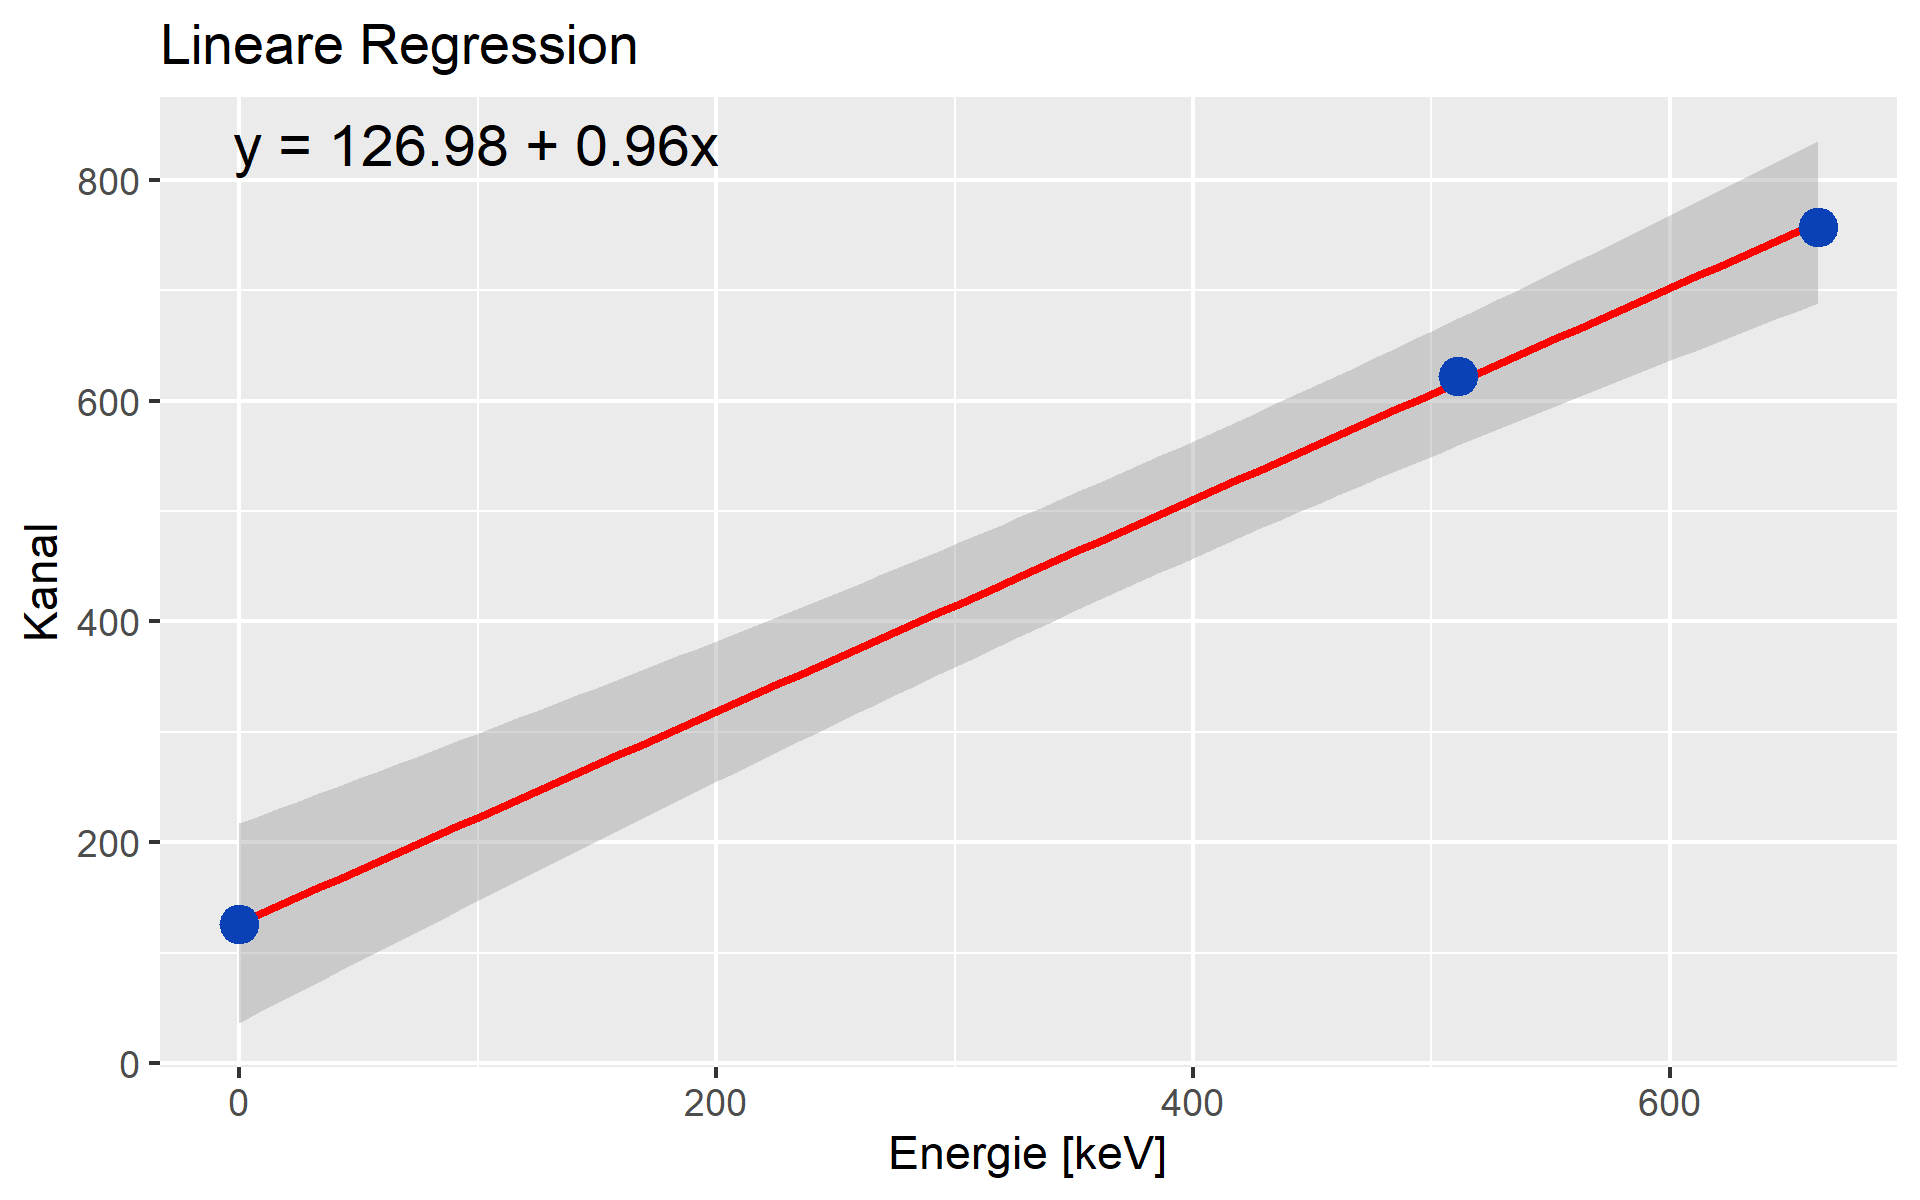
\includegraphics[width=.5\textwidth]{EichLinFit.png}
					\caption{Linearer Fit an die gemessenen Energien der Gammaquellen mit R}
					\label{fig:EichLinFit}
			  \end{figure}

		  \section{Bestimmung der Elektron-Ruhemasse}

		  \section{Vergleich mit Klein–Nishina Formel}



    \chapter{Fazit}

	\listoffigures
    \addcontentsline{toc}{chapter}{\listfigurename}

	\begin{thebibliography}{111} \addcontentsline{toc}{chapter}{Literaturverzeichnis}
		\bibitem{Anleitung}
		AR Dr. Jens Sören Lange, \glqq Praktikumsanleitung zu \glq Versuch: Comptoneffekt\grq \grqq{}, 2015.


	\end{thebibliography}


	\chapter*{Anhang} \label{ch:Anhang}
    \addcontentsline{toc}{chapter}{Anhang}
    \FloatBarrier



	
		\begin{figure}[ht]
			\centering
			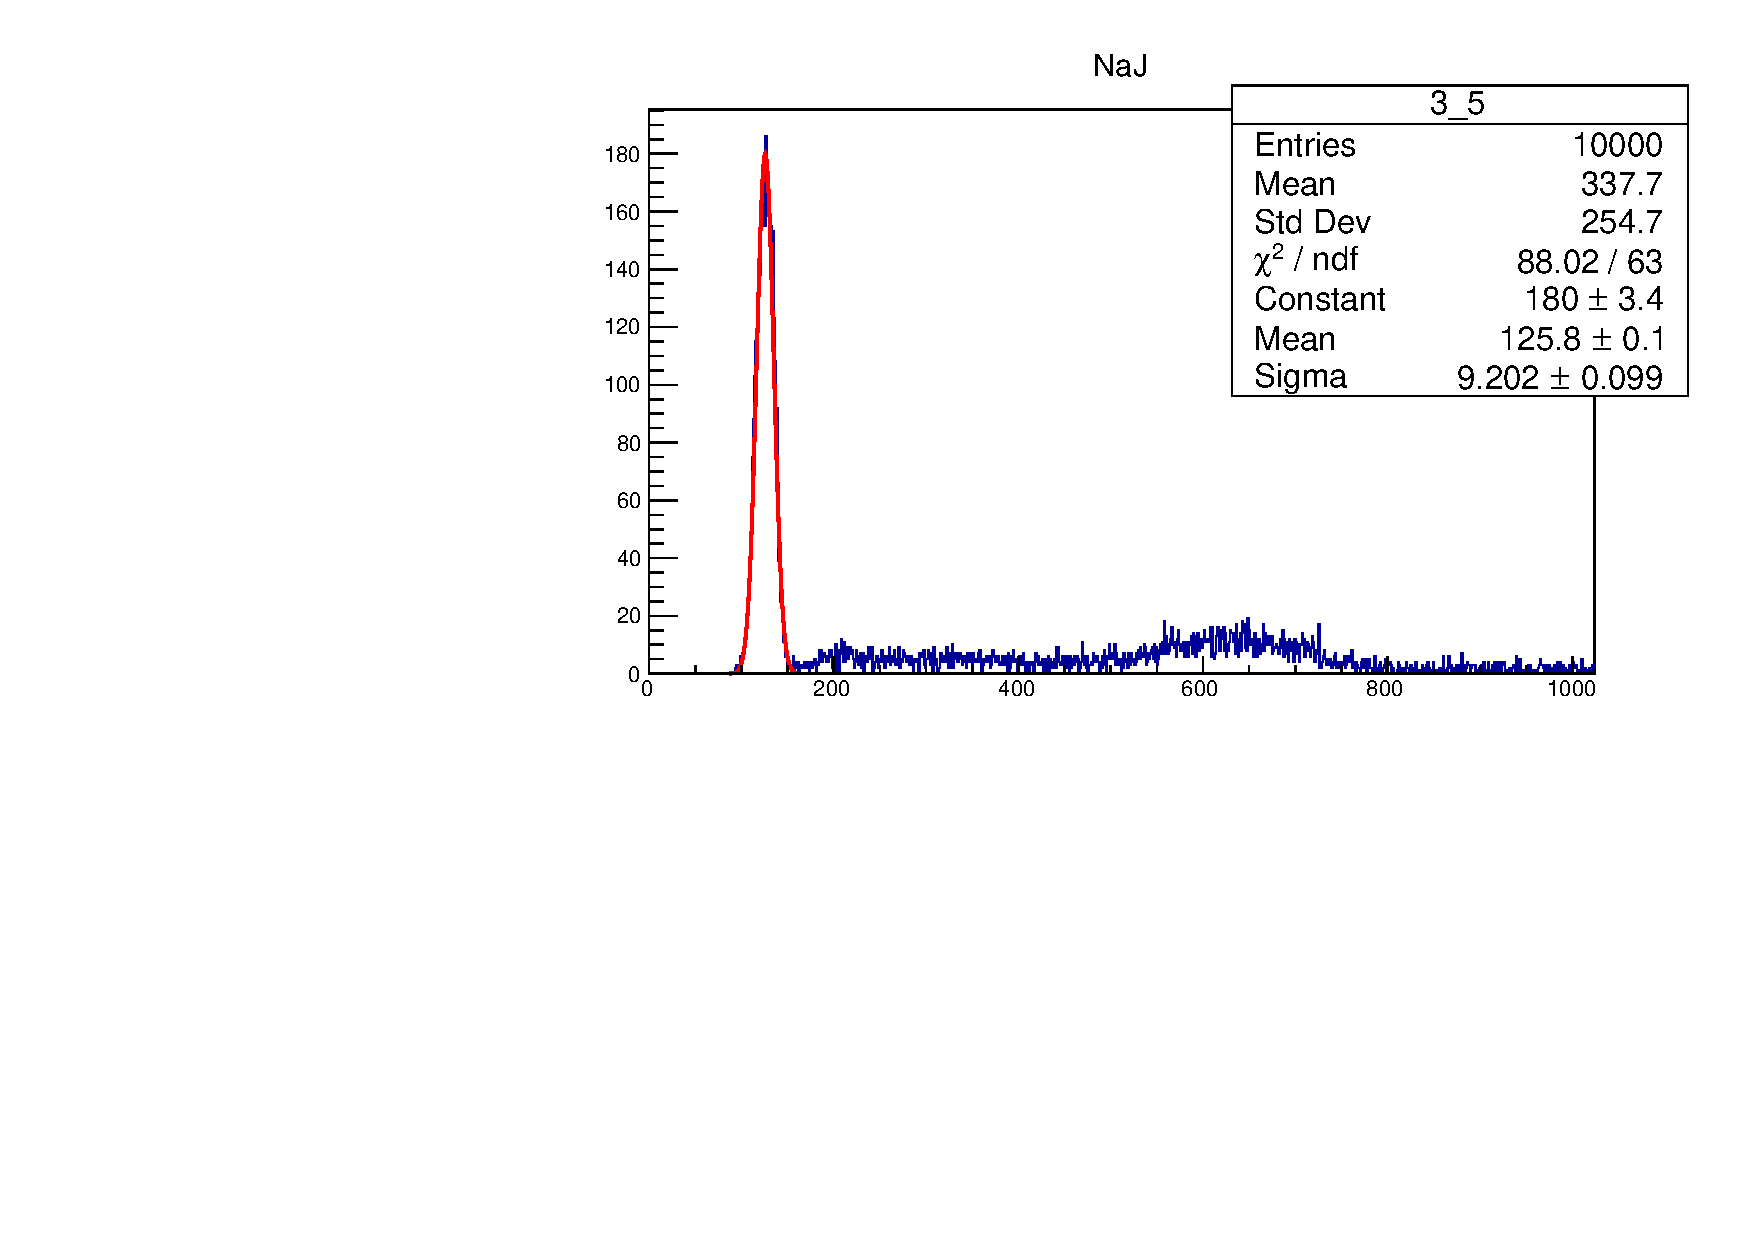
\includegraphics[page=1,width=.4\textwidth]{eich_pedestal2}
			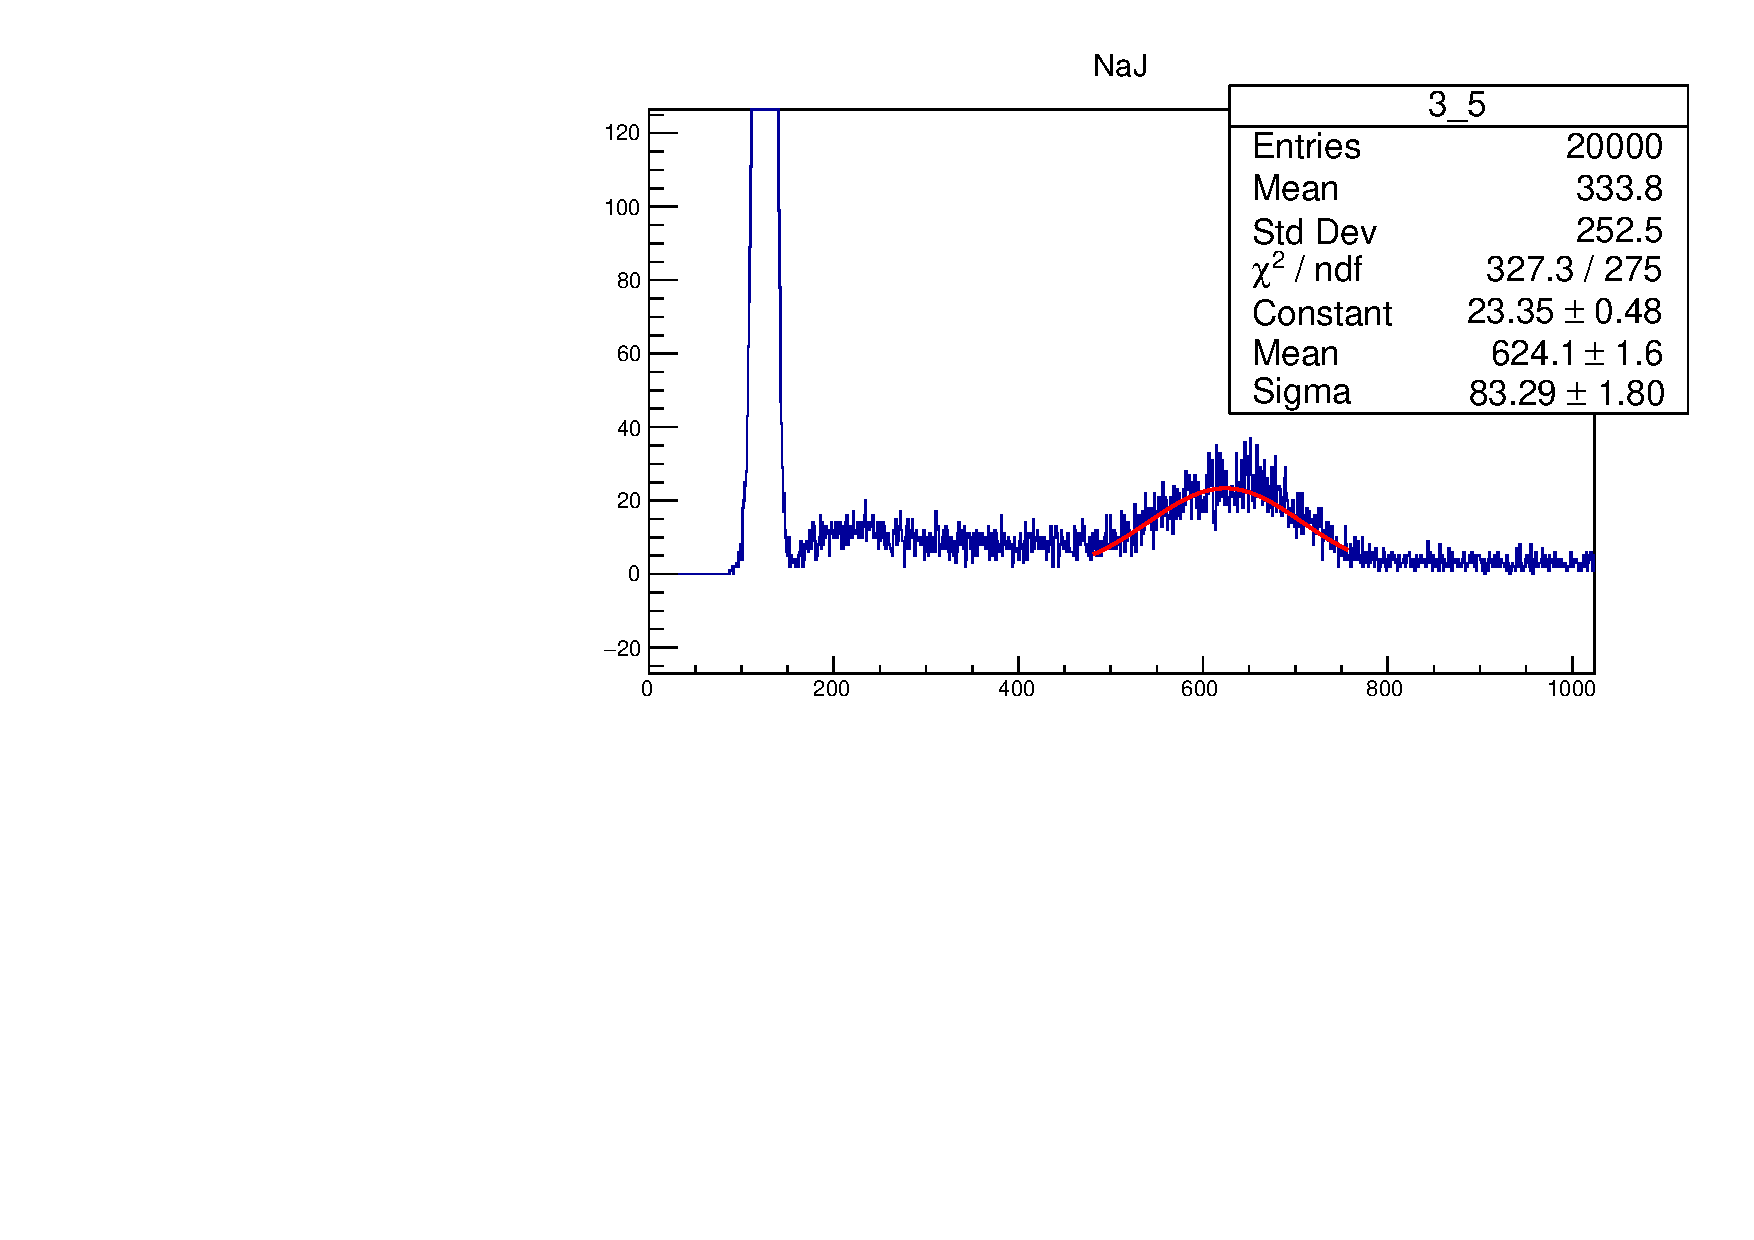
\includegraphics[page=1,width=.4\textwidth]{eich_na2}\hspace*{.25\textwidth}%
			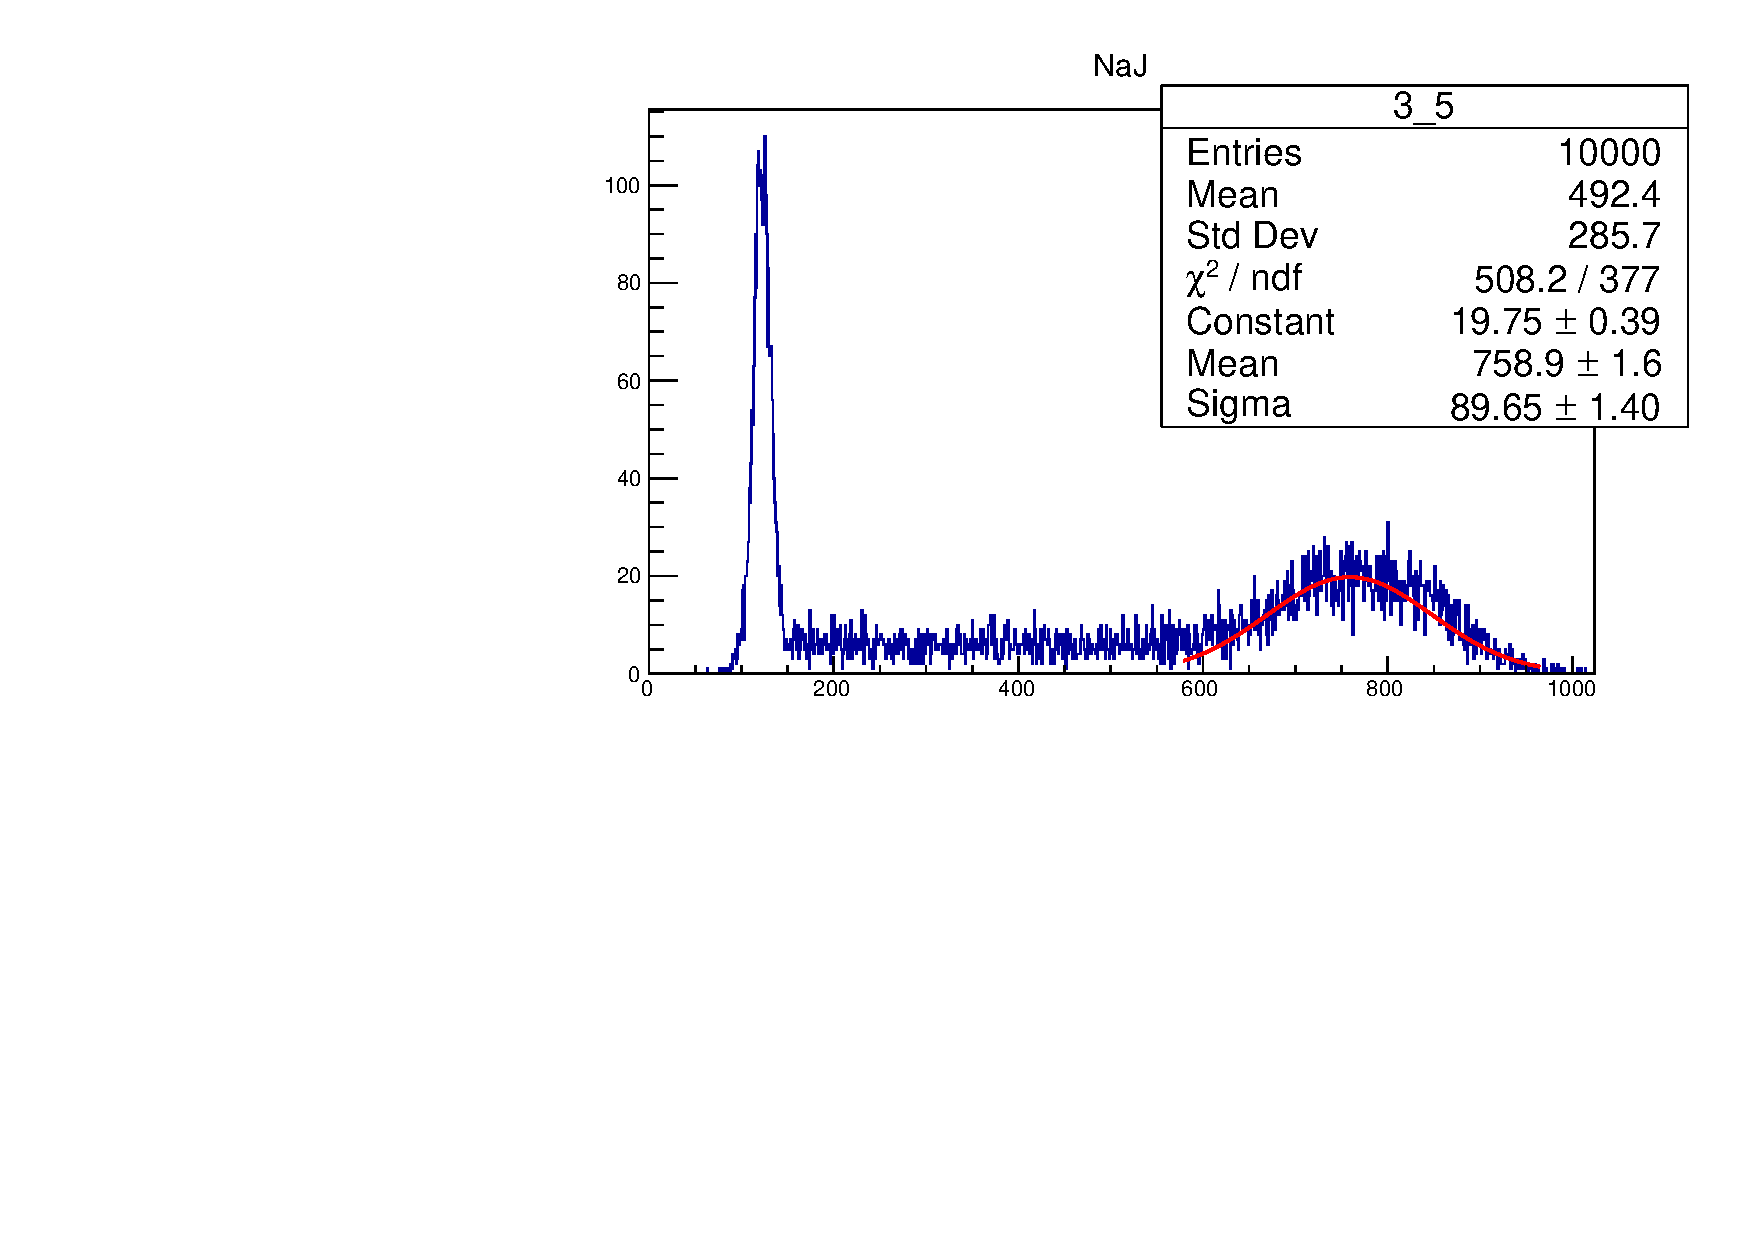
\includegraphics[page=1,width=.4\textwidth]{eich_cs}
			
			\caption{Eichmessung: Oben Pedestal, unten links: Na, unten rechts: Cs}
			\label{fig:Eichmessung}
		\end{figure}


\end{document}
